\documentclass{article}


%%%%%%%%%%%%%%%%%%%%%%%%%%%%%%%%%%%%%%%%%%%%%%%%%%%%%%%%%%%%%%%%%%%%%%%%%
\pagestyle{plain}                                                      %%
%%%%%%%%%% EXACT 1in MARGINS %%%%%%%                                   %%
\setlength{\textwidth}{6.5in}     %%                                   %%
\setlength{\oddsidemargin}{0in}   %% (It is recommended that you       %%
\setlength{\evensidemargin}{0in}  %%  not change these parameters,     %%
\setlength{\textheight}{8.5in}    %%  at the risk of having your       %%
\setlength{\topmargin}{0in}       %%  proposal dismissed on the basis  %%
\setlength{\headheight}{0in}      %%  of incorrect formatting!!!)      %%
\setlength{\headsep}{0in}         %%                                   %%
\setlength{\footskip}{.5in}       %%                                   %%
%%%%%%%%%%%%%%%%%%%%%%%%%%%%%%%%%%%%                                   %%
\newcommand{\required}[1]{\section*{\hfil #1\hfil}}                    %%
\renewcommand{\refname}{\hfil References Cited\hfil}                   %%
\bibliographystyle{plain}                                              %%
%%%%%%%%%%%%%%%%%%%%%%%%%%%%%%%%%%%%%%%%%%%%%%%%%%%%%%%%%%%%%%%%%%%%%%%%%

\usepackage{graphicx}

\pagestyle{plain}

\begin{document}

\large

\vbox{}
\begin{figure}[!ht]
%\hspace{-4mm}

\includegraphics[width=8cm]{logo.png}
\vspace{4mm}
\end{figure}

\centerline{\huge \bf Geometry Editor}
\vspace{6mm}
\noindent
This help will guide you through NCLab's Geometry Editor (GE).

\subsection*{Copyright and Restricted Use Notice}

The Geometry Editor (GE) is part of the Networked Computing Laboratory (NCLab) and its sole purpose is to facilitate the definition of computational domains in NCLab. GE is a closed-source code that is copyrighted by FEMhub Inc. Copying and any use outside of NCLab is strictly prohibited.

\subsection*{Launching GE}

GE can be launched from any Python worksheet in NCLab by issuing 

\begin{verbatim}
lab.geometry_editor().
\end{verbatim}
After GE launches, right-click in the work area and a menu will appear:\\

\begin{figure}[!ht]
\begin{center}
%\hspace{-4mm}
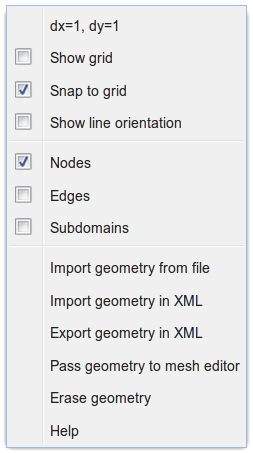
\includegraphics[width=4.5cm]{ge-menu.png}
\end{center}
\vspace{-4mm}
\caption{Geometry Editor's menu.}
\end{figure}


\subsection*{Overview of Menu Functions}

In the order of appearance, the menu functions do the following:
\begin{itemize}
\item Grid spacing: Sets grid spacing in the x and y directions.
\item Show grid: Turns on and off grid display.
\item Snap to grid: Facilitates entering of nodes using intersection of grid lines..
\item Show line orientation: By default, each edge is oriented from the older node (lower index) to the newer one (higher index). If this checkbox is on, edge orientations are shown using arrows.  
\item Nodes: Operate on nodes. In this mode one can:
\begin{itemize}
\item add new nodes (CTRL + click), 
\item move nodes, 
\item edit nodes (double-click), 
\item delete nodes.
\end{itemize}
\item Edges: Operate on edges. In this mode one can:
\begin{itemize}
\item add new edges (hold CTRL down and move mouse to get suggestions, click to select), 
\item turn edges into circular arcs,
\item assign markers to edges,
\item flip edge orientations.
\end{itemize}
\item Subdomains: Operate on subdomains. In this mode on can assign markers to subdomains. 
\item Import geometry from file: Imports geometry from a file on the hard disk.
\item Import geometry in XML: Imports geometry via pasting a text in XML format.
\item Export geometry in XML: Exports geometry for copying and pasting in XML format.
\item Pass geometry to mesh editor: Launches Mesh Editor with the current geometry imported.
\item Erase geometry: Discards current geometry.
\item Help: Launches this Help.
\end{itemize}

\subsection*{GE Workflow}

Geometry preparation typically takes the following steps: 
\begin{enumerate}
\item Import existing geometry in XML (optional).
\item Create new nodes.
\item Connect nodes with edges. 
\item Flip edge orientations as needed.
\item Deform some edges to circular arcs as needed.
\item Subdivide some edges uniformly as needed.
\item Assign markers to edges.
\item Assign markers to subdomains (double-click on a domain in Subdomains mode).
\item Export geometry in XML (optional).
\item Pass geometry to Mesh Editor.
\end{enumerate}

\subsection*{Operating on Nodes}

Right-click in the work area and in the menu choose Nodes. If you want to enter nodes at the intersections of grid lines only, check Snap to grid, otherwise leave this unchecked. Press CTRL and move the mouse over the work area. Node positions will be suggested, either at the mouse tip or at the closest intersection of grid lines, depending on the status of Snap to grid. Left mouse click will insert a node into the domain. Nodes can be dragged by mouse.  Any node can be double-clicked to edit its coordinates manually or delete it.

\subsection*{Operating on Edges}

Switch to Edges in the menu. Press CTRL and move the mouse over the work area. Edges will be suggested (based on minimum distance of their end-points from the mouse). If GE does not suggest an edge that you want, you can force it by clicking on its vertices. Left click will add an edge to the domain. Any edge can be double-clicked to flip its orientation, change it to circular arc, assign a marker, or delete it. Circular arcs are defined via end points and a central angle. 

\subsection*{Operating on Subdomains}

Switch to Subdomains in the menu. When you move the mouse over the geometry, subdomains will be highlighted. Any subdomain can be double-clicked to add a marker or delete it.

\subsection*{XML Geometry File Format}

The following is a simple example of a geometry with six nodes, seven edges of which two are 45-degree circular arcs,  and two subdomains. The <nodes> section is self-explanatory, just remember that indices start at 0. In the <edges> section, each edge is defined using a pair of node indices, an angle and a marker. If the angle is 0, then this is a straight edge, otherwise it is a circular arc. In the <subdomains> section, each subdomain is defined using a point that is inside, and a marker. 

\begin{verbatim}
<geometry>
  <nodes>
    <node x='0.15' y='-0.05' id='0'/>
    <node x='0.15' y='0.1' id='1'/>
    <node x='-0.15' y='0.1' id='2'/>
    <node x='-0.15' y='-0.05' id='3'/>
    <node x='0' y='-0.05' id='4'/>
    <node x='0' y='0.1' id='5'/>
  </nodes>
  <edges>
    <edge start='2' end='5' angle='0' marker='top-left'/>
    <edge start='2' end='3' angle='45' marker='left-arc'/>
    <edge start='4' end='3' angle='0' marker='bottom-left'/>
    <edge start='4' end='5' angle='0' marker='middle-vertical'/>
    <edge start='0' end='4' angle='0' marker='bottom-right'/>
    <edge start='1' end='0' angle='45' marker='right-arc'/>
    <edge start='5' end='1' angle='0' marker='top-right'/>
  </edges>
  <subdomains>
    <subdomain x="-0.075" y="0.025" marker="left"/>
    <subdomain x="0.075" y="0.025" marker="right"/>
  </subdomains>
</geometry>
\end{verbatim}

\subsection*{Known Bugs}

No known bugs at this time. Please report bugs to {\tt nclab-user@googlegroups.com}.
\end{document}

